\section{Lektion 15-02-2018}

\begin{enumerate}
	\item Stående bølger
	\item Geometrisk rumakustik
	\item Refleksion
	\item Diffraktion
	\item Statistisk rumakustik
	\item Absorptionskoeffficienter
\end{enumerate}

\begin{mdframed}[style=exampledefault]
	\begin{itemize}
		\item \textbf{Pensum:} 
		\begin{enumerate}
			\item Master Handbook of Acoustics, ch. 6, 7, 11, 13
			\item Elektroakustik, TAS,  p. 89-96
		\end{enumerate}
		\item \textbf{Opgaver:} 
		\begin{enumerate}
			\item Lyd og Akustik - Lektion 4 - opgaver og øvelser
		\end{enumerate}
	\end{itemize}
\end{mdframed}

\subsection{Stående bølger}
Et retvinklet rum vil have et system af egenfrekvenser. Her vil plane bølger spejles så de understøtter bestemte frekvenser. Dette sker gennem konstruktiv interferens. \\

Den laveste frekvens hvor der kan dannes resonans i en akseretning har en bølgelængde på halvdelen af længdedimensionen ($L_x$, $L_y$ og $L_z$). Trykbølgen reflekteres ved væggen og refleksionen kan derfor understøtte den efterfølgende bølgefront.
\begin{itemize}
	\item Ved \SI{5}{\meter} afstand mellem to vægge er den lavest mulige resonans $f_0 = \SI{34}{\hertz}$. Hertil kommer også resonans ved de harmoniske frekvenser på \SI{68}{\hertz}, \SI{102}{\hertz}, ... Tilsvarende gælder for de andre akseretninger.
\end{itemize}
Der er mulighed for stående bølger som involverer fire eller seks vægge.
Dette beskrives ved at to eller tre værdier af index ($n_x$, $n_y$ og $n_z$) er forskellige fra nul. 
De tre indeksværdier kombineres til et enkelt ved at udnytte at N er den højest mulige værdi. Herved kan resonanserne plottes som
funktion af et fælles indeks \textit{n}.\\

Modellen gælder indtil frekvenser hvor usikkerheden på længderetningen
bliver sammenlignelig med bølgelængden. 
Det kan vises at den øvre grænse er i cirka \SI{550}{\hertz} for
et normalt beboelsesrum hvorved det enkelte indeks er begrænset til området $n = 0$ ... $7$.

\begin{figure} [H]
	\centering
	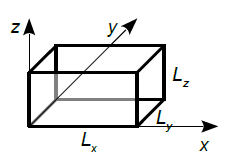
\includegraphics[width=.4\linewidth]{graphics/13.png}
	\caption{Plane lydbølger kan eksistere i et rektangulært rum.}
	\label{fig:13}
\end{figure}
\noindent\textbf{Resonanser}
\begin{equation}
f_n = \sqrt{\left(\dfrac{n_x c}{2 L_x}\right)^2 + \left(\dfrac{n_y c}{2 L_y}\right)^2 + \left(\dfrac{n_z c}{2 L_z}\right)^2}
\end{equation}

\noindent\textbf{Øvre grænse}
\begin{equation}
f_{max}\approx \dfrac{c}{2\pi \Delta L}
\end{equation}

\begin{equation}
N \approx 1 +\dfrac{V}{S \Delta L}
\end{equation}

\begin{description}
	\item[$V$] rummets volume $m^3$
	\item[$\Delta L$] længdedimensionen
	\item[$S$] lydabsorberende areal
\end{description}
\newpage
\begin{itemize}
	\item Ved lave frekvenser er det let at adskille de enkelte resonanser.
	\item Ved højere frekvenser rykker resonanserne sammen og flere resonanser vil blive aktiveret i større eller mindre grad af en stationær tone. 
	\item Når centerfrekvensen af et antal	resonanser falder indenfor båndbredden af det enkelte filter er det umuligt at skelne mellem
	egenfrekvenserne.
	\item Grænsefrekvensen mellem det område hvor de enkelte resonanser kan erkendes og det område	hvor de er smeltet sammen kaldes for Schröder frekvensen. 
	\item Findes fra rummets volumen $V$ og efterklangstid $T_{60}$. Teorien antager at der vil ligge mindst	tre resonanser indenfor det midterste filters $–3 \si{\decibel}$ båndbredde.
\end{itemize}

\begin{equation}
f_s = 2000 \sqrt{\dfrac{T_{60}}{V}}
\end{equation}

\begin{itemize}
	\item Rummets resonanser er ansvarlig for efterklangen i rummet.
	\item En højttaler udsender	et støjsignal der indeholder alle frekvenser så samtlige resonanser i rummet aktiveres. 
	\item Når lydniveauet er blevet konstant standses lyden fra højttaleren og lydniveauet aftager i takt med at lydenergien absorberes i tæpper, træpaneler og vinduer samt luften selv.
	\item Efterklangstiden $T_{60}$ er defineret som tiden indtil signalet er reduceret til \SI{-60}{\decibel} af det oprindelige niveau.
	\item Resonanserne kan beskrives ved dæmpede svingninger der fra filterteorien repræsenteres af et anden-ordens filter for hver resonans.
\end{itemize}

\begin{equation}
H(s)=\sum_{n=0}^{N}\dfrac{C_n}{s^2+2d_n\omega_n s+\omega_n^2}
\end{equation}

\begin{equation}
h(t)=\sum_{n=0}^{N} C_n \sin(\omega t) \exp(-d_n\omega_n t)
\end{equation}

\subsection{Geometrisk rumakustik}
En lydbølge fra lydgiveren udbredes med en konstant hastighed i alle retninger. 
En lytter i nogen afstand fra lydgiveren vil modtage lydbølgen efter en forsinkelse $t_D$ på cirka $3 \si{\milli\second}$ per meter.\\

Lydbølgen vil fortsætte sin udbredelse indtil den rammer en flade i rummet hvor den reflekteres og den reflekterede bølgefront kan derfor nå frem til lytteren efter yderligere forsinkelse. 
Øret vil modtage et system af lydbølger der både beskriver det materiale der lyttes på og det rum lydkilden og personen befinder sig i.
\subsubsection{Refleksion}
\begin{itemize}
	\item Et rums impulsrespons kan beregnes ved at følge de veje som refleksionerne vil løbe. Resultatet bliver kun en tilnærmelse uanset hvor omhyggeligt der beregnes.
	\item En refleksion forløber ikke med stor præcision. Der opstår en udtværing af det reflekterede signals retning som nu spredes i enhver retning og ikke alene er givet af signalets ind- og udfaldsvinkler.
	\item Den direkte spejling står for cirka 80 \% af energien i den
	indfaldne bølgefront og den diffuse udstråling i enhver retning står for den resterende energi.
	\item Som model af den diffuse stråling anvendes statistiske metoder for at ændre lidt på refleksionens retning i forhold til en direkte spejling.
\end{itemize}

\begin{figure} [H]
	\centering
	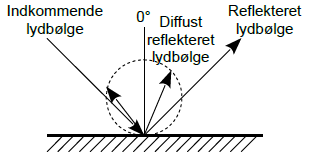
\includegraphics[width=.55\linewidth]{graphics/14.png}
	\caption{En lydbølges refleksioner sker både som en direkte spejling af lydbølgen og som en diffus lydbølge.}
	\label{fig:14}
\end{figure}

\subsubsection{Diffraktion}
Hvordan lydbølger bøjes af små forhindringer og hvordan lydbølger udbredes efter små åbninger. 

\begin{itemize}
	\item En forhindring meget smallere end lydbølgen gør at lydbølgen kan passere uden at blive synderligt forstyrret.
	\item En forhindring større end lydbølgen vil resultere i at der bliver kastet en skygge (casts a shadow) der vil  blive bestrålet fra kilder, der går forbi forhindringen.
\end{itemize}

\begin{figure} [H]
	\centering
	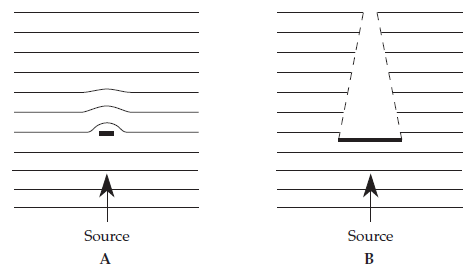
\includegraphics[width=.5\linewidth]{graphics/15.png}
	\caption{Diffraktion er wavelength-dependent.}
	\label{fig:15}
\end{figure}

\begin{itemize}
	\item Diffraktionen afhænger af	den relative størrelse af åbningen. 
	\item En stor åbning med hensyn til bølgelængde tillader lydbølger at gå igennem med en lille forstyrrelse. 
	\begin{itemize}
		\item Disse bølgefronter virker som nye kilder, der udstråler lydenergi i skyggezonen.
	\end{itemize}
	\item Hvis åbningen er lille i forhold til bølgelængden, vil de små bølgefronter, der trænger ind i åbningen virke som punktkilder.
	\begin{itemize}
		\item Disse små bølgefronter vil udstråle et halvkugleformet lydfelt ind i skyggezonen.
	\end{itemize} 
\end{itemize}

\begin{figure} [H]
	\centering
	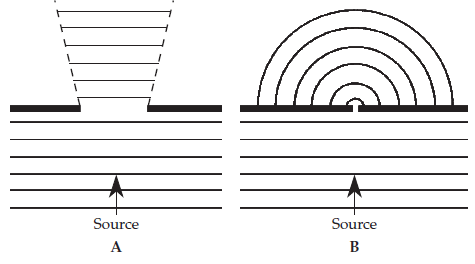
\includegraphics[width=.5\linewidth]{graphics/16.png}
	\caption{Lydbølger der rammer en barriere med en åbning.}
	\label{fig:16}
\end{figure}


\subsection{Statistisk rumakustik}
\begin{itemize}
	\item Antager at lydenergien er konstant overalt i rummet.
	\item \textbf{Sabines formel} for efterklangstiden $T_{60}$ som funktion af rummets volumen V og det lydabsorberende areal S.
\end{itemize}

\begin{equation}
T_{60} = \ln(10^6)\dfrac{4V}{S c} = 55.3\dfrac{V}{S c} = 0.16\dfrac{V}{S}
\end{equation}

\begin{itemize}
	\item For lyddæmpede rum giver Sabines formel en efterklangstid selv om der ikke er refleksioner. En modificeret udgave af Sabines formel blev udledt af Eyring.
	\item \textbf{Eyrings formel} er modificeret ud fra geometriske betragtninger.
\end{itemize}

\begin{equation}
T_{60} = 0.16\dfrac{V}{4 m V-S\ln(1-\alpha)}
\end{equation}

\begin{description}
	\item[$\alpha$] $=\frac{1}{S}\sum_{n}^{}S_n \alpha_n$
	\item[$m$] $\approx0.0011 m^{–1}$ ved \SI{1}{\kilo\hertz}, \SI{20}{\degreeCelsius} og 60 \% relativ luftfugtighed
\end{description}
\textit{m} kan ignoreres for mindre rum og rum med ringe dæmpning bliver formlen lig med Sabines.

\subsection{Absorptionskoeffficienter}
\begin{itemize}
	\item Typisk opsætning af lydabsorberende skumplast og Rockwool er direkte på en hård betonvæg.
	\item Tykkelsen er afgørende for hvor lave frekvenser der kan dæmpes da partikelhastigheden er nul ved væggen så det er kun	ved høje frekvenser at der er bevægelse i luften inde i materialet.
	\item For at opnå større absorption ved lave frekvenser kan benyttes absorbere baseret på en membran.
	\begin{itemize}
		\item De består af en plade eller film af træ, plast eller metal som lydtrykket får til at vibrere.
		\item Derved skal luften bag ved membranen også svinge så luften presses igennem det absorberende materiale.
	\end{itemize}
\end{itemize}

\subsection{Opgaver}
\subsubsection{1.}
Beregn de første 10 rum-resonanser i lyttestuen. Angiv hvilke der er aksiale. Beregn også Schröder-frekvensen og estimer efterklangstiden T60.
\begin{figure} [H]
	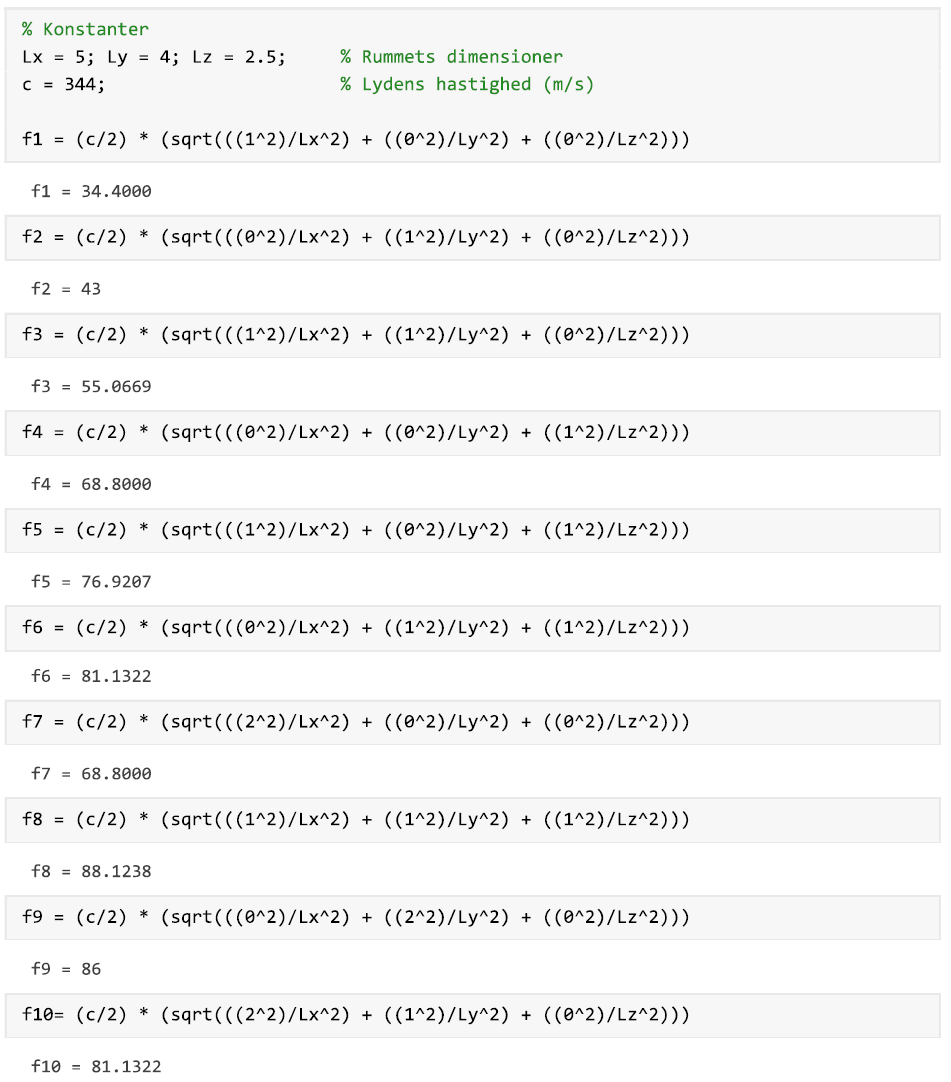
\includegraphics[width=\linewidth]{graphics/32.png}
\end{figure}
\newpage
\begin{figure} [H]
	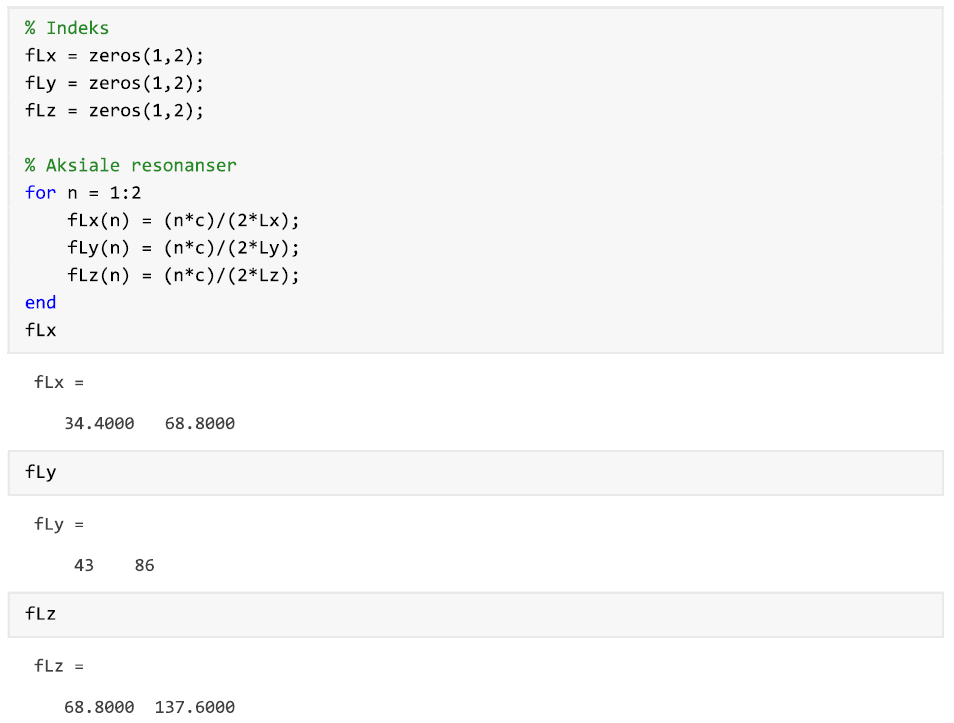
\includegraphics[width=\linewidth]{graphics/33.png}
\end{figure}
\begin{figure} [H]
	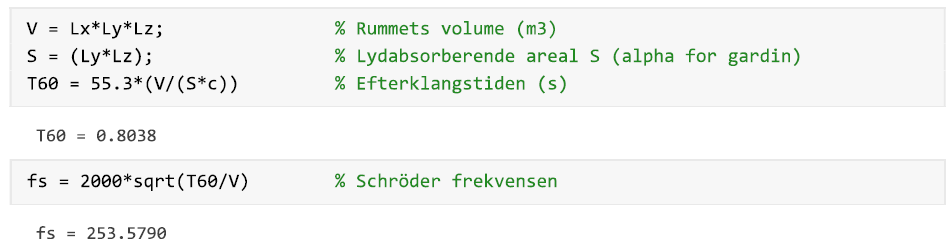
\includegraphics[width=\linewidth]{graphics/34.png}
\end{figure}
\subsubsection{2.}
Giv et bud på delay og relativ styrke for alle 1. ordens reflektioner (for faste kilde/lytter placeringer). Tegn impulsresponsen som søjler langs en tidsakse, hvor lyddæmpningen medtages efter afstandsreglen og eventuelt en vurdering af dæmpningen ved refleksion i fx loftplader.
\subsubsection{3.}
Beregning af efterklangstiden T60 efter Sabine for forskellige rum. Vurdering af absorption ved brug af kurverne i \href{http://www.torean.dk/artikel/Elektroakustik.pdf}{Elektroakustik,} side 50-51 eller "Report 2 – Absorber" fra Campus, eller formler fundet på nettet.
\begin{figure} [H]
	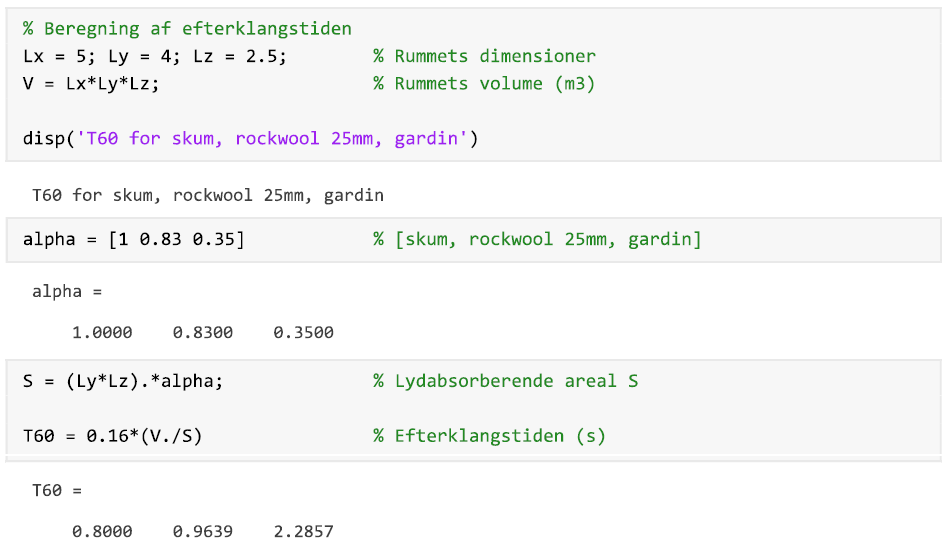
\includegraphics[width=\linewidth]{graphics/35.png}
\end{figure}

\subsubsection{4.}
Bestem de rumakustiske parametre T60, EDT, og C80 ud fra impulsresponsen i filen roomir.mat.

\begin{figure} [H]
	\centering
	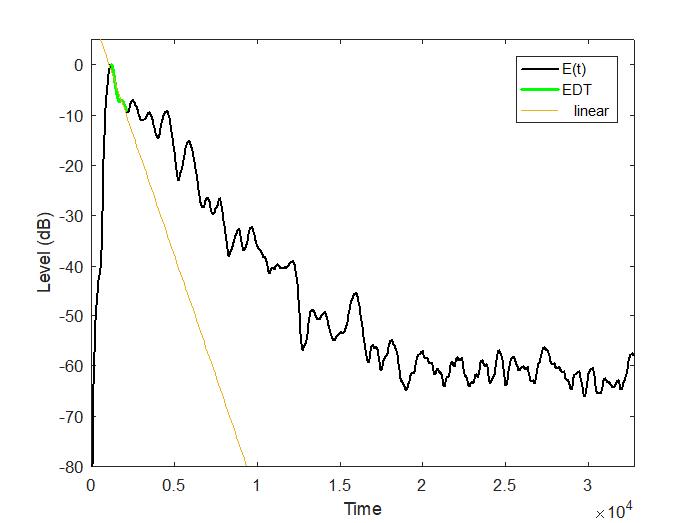
\includegraphics[width=\linewidth]{graphics/50.png}
	\caption{Bestemmelse af EDT.}
	\label{fig:50}
\end{figure}


\begin{figure} [H]
	\centering
	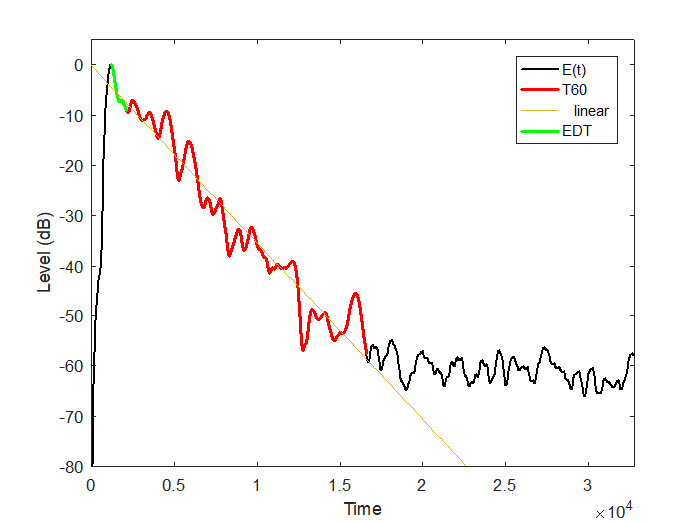
\includegraphics[width=\linewidth]{graphics/51.png}
	\caption{Bestemmelse af T60.}
	\label{fig:51}
\end{figure}


\begin{figure} [H]
	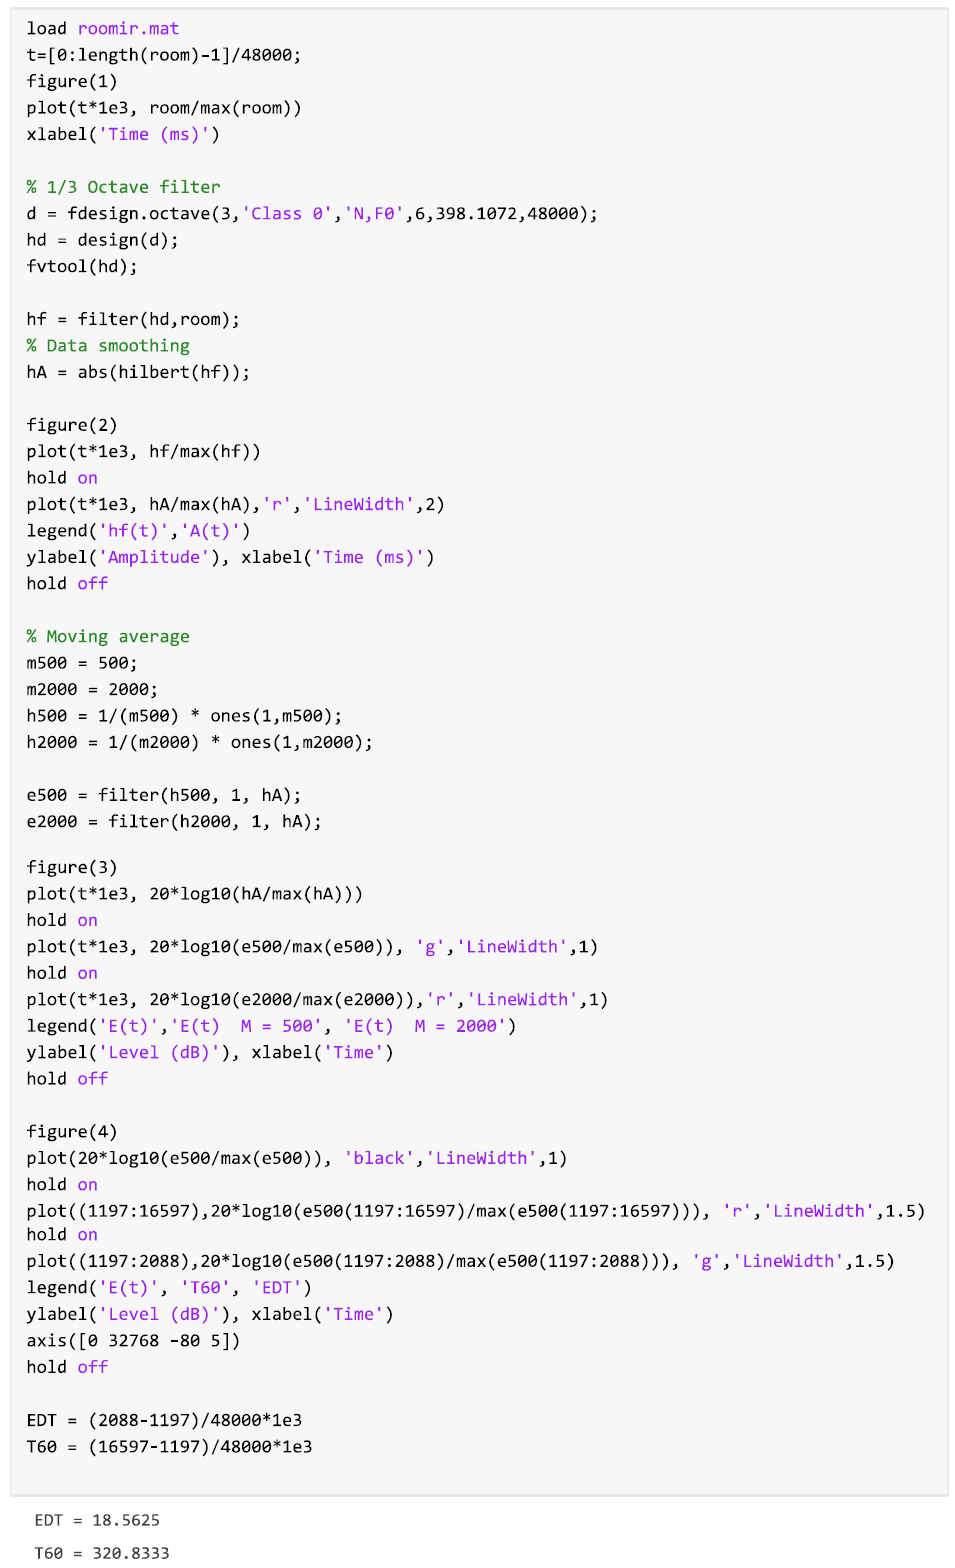
\includegraphics[width=\linewidth]{graphics/52.png}
\end{figure}


\subsection{Øvelser}
\subsubsection{Øvelse 4.1}
Opstilling af en højttaler og eftersøgning efter resonansfrekvenserne fra opg. 1. Bestemmelse af tryk-maksima og sammenhold det med teorien for trykmaksima i hjørnet. Sammenligning med den beregnede øvre grænse $f_{MAX}$ eller $N$ for betydningen af afvigelser fra et rektangulært rum.

\subsubsection{Øvelse 4.2}
Måling af T60 ved en højttaler med hvid/rosa støj, der pludseligt afbrydes, eller ved et klap i hænderne: Klasseværelset, musiklytterummet (med en skrå væg), efterklangsrummet i kælderen og det lyddøde rum. Relater målingerne til de beregnede resultater fra opg. 3.
